\chapter{Resultados}
\label{resultados}

La evaluación de resultados se realizó utilizando la opinión de los médicos y 
también utilizando los diagramas como herramienta evaluadora.

Cada caso preprocesado se almacenó en un servidor y está disponible en la siguiente
dirección: \url{www.casi.dais.mx}.

El código fuente que se generó está disponible en línea bajo un controlador de
versiones en el repositorio: \texttt{github.com/omartrinidad/mammograms}.

\begin{figure}[h!]
  \begin{center}
    \hspace{\fill}
    \subfloat[12 bits]{
    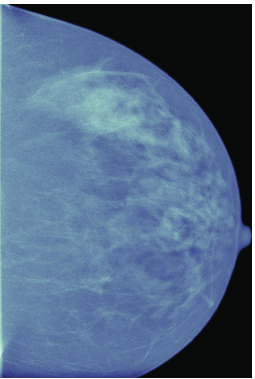
\includegraphics[width=0.30\columnwidth]{images/compressed-mammogram-8bits}
    }
    \hfill
    \subfloat[16 bits]{
    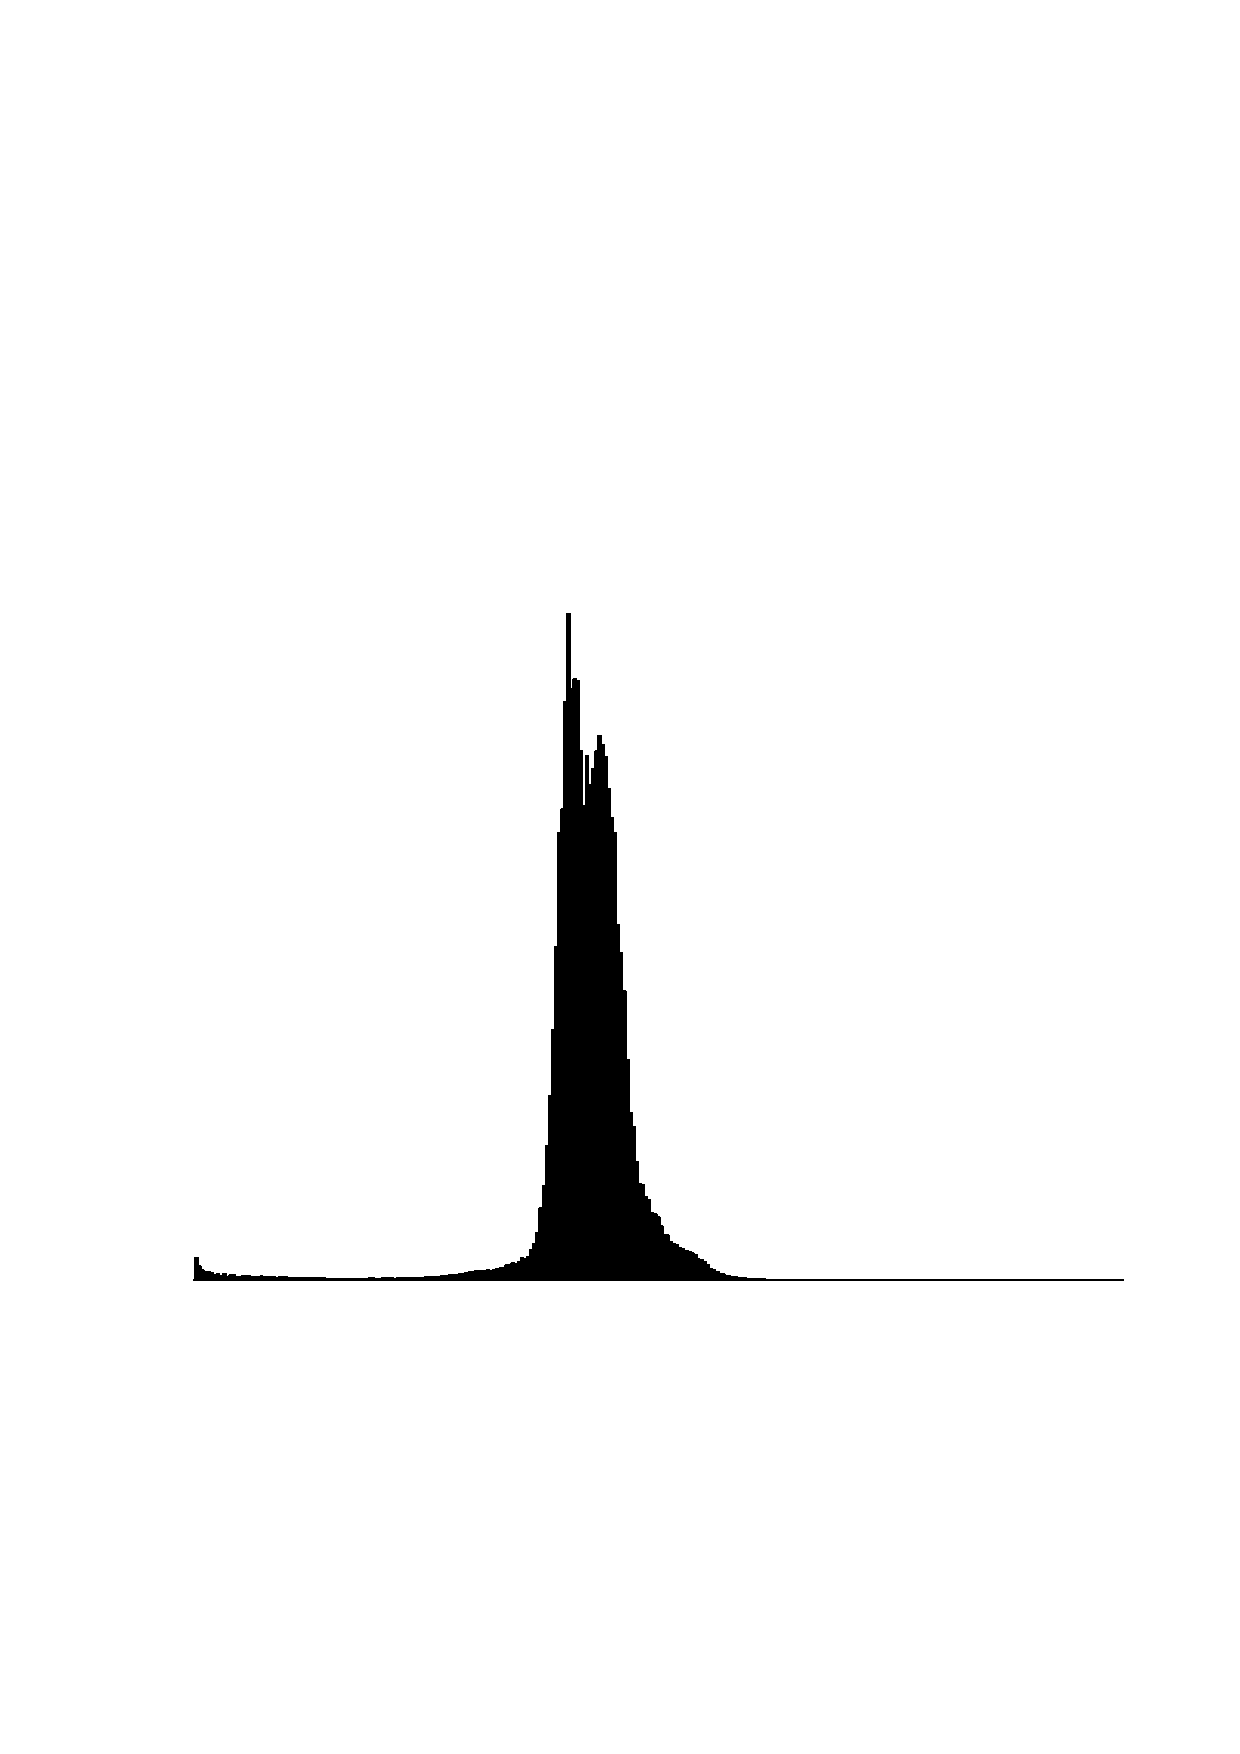
\includegraphics[width=0.30\columnwidth]{images/compressed-mammogram-histogram}
    }
    \hspace{\fill}
  \caption[Compressed 8-bits mammogram and histogram]{This description appears 
  in above of the image.}
  \end{center}
  \label{8bits} 
\end{figure}


